\chapter{Comunicaciones multiusuario}
\section{Introducción}
En este capítulo se abordan los problemas y métodos modernos para aprovechar al máximo el canal en comunicaciones multiusuarios.\\

\section{MULTIPLEXACIÓN POR DIVISIÓN DE TIEMPO (TDM). LA REVOLUCIÓN PCM }
Veámos  el problema que dió origen a  aparición del Multiplexado por División de Tiempo (TDM) en los años 60: Todos los hogares soñaban con tener un teléfono, pero los costos del servicio no estaban al alcance de todos. La telefonía era analogica y establecer una llamada entre dos personas requería establecer una conexión física, alambrada entre ellas, como se muestra en la siguiente figura. \\

\begin{figure}[h!]
	\captionsetup{justification = raggedright, singlelinecheck = false}
	\caption{Central local} 
	\centering
	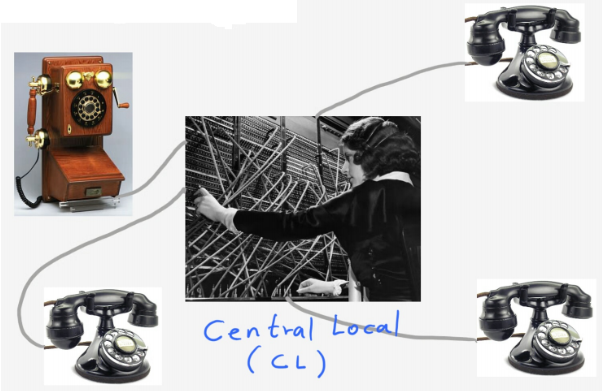
\includegraphics[scale=0.8]{Imagenes/Central-local.png}
	\label{fig:Central}
	%		\captionsetup{justification=raggedright,font={scriptsize,bf,it}}
	%		\caption*{fuente: http://superkuh.com/rtlsdr.html}
\end{figure}

\vspace{200px}
\begin{figure}[h!]
	\captionsetup{justification = raggedright, singlelinecheck = false}
	\caption{Central de transito} 
	\centering
	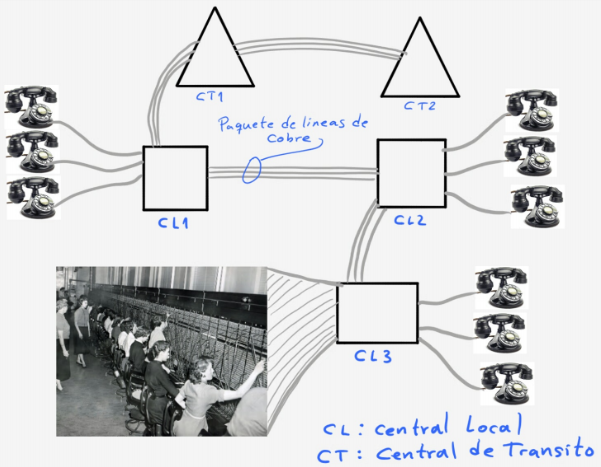
\includegraphics[scale=0.8]{Imagenes/Central-transito.png}
	\label{fig:Central-transito}
	%		\captionsetup{justification=raggedright,font={scriptsize,bf,it}}
	%		\caption*{fuente: http://superkuh.com/rtlsdr.html}
\end{figure}

El problema: se volvió insostenible el creciente número de operadoras en las centrales telefónicas, sin que bajarán sensiblemente los costos de conexión. La telefonía seguía siendo solo para los elites. La UIT se propuso impulsar una revolución para lograr que cada hogar tuviese un teléfono. Esa es conocida como la revolución PCM (Pulse Code Modulation). La idea es que la voz de cada llamada se convierte a PCM, las centrales telefónicas cambiarían la conmutación manual por la conmutación por circuitos que se podía realizar de manera automática, por medios computarizados. Pero el mayor avance consistió en lograr que cada línea que une dos centrales telefónicas, que antes podía llevar solo una llamada en un momento determinado, pudiera ahora llevar cientos de llamadas multiplexadas por división de tiempo. \\

La siguiente figura muestra resume el principio de TDM.

\begin{figure}[h!]
	\captionsetup{justification = raggedright, singlelinecheck = false}
	\caption{Ejemplo de TDM} 
	\centering
	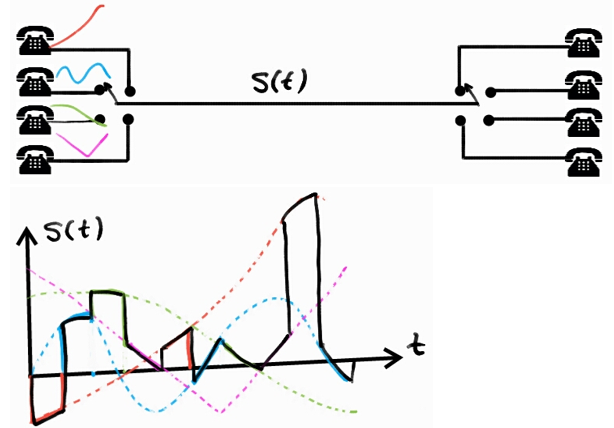
\includegraphics[scale=0.5]{Imagenes/Telefono.PNG}
	\label{fig:Telefono}
	%	\captionsetup{justification=raggedright,font={scriptsize,bf,it}}
	%	\caption*{fuente: \textcolor{
	%Orange}{Tomada de Wikipedia}}
\end{figure}

Como puede verse, entre los dos puntos comunicantes viaja una sola señal, en cada uno de los teléfonos receptores llega una señal que es una versión PAM (Pulse Amplitud Modulation) de la emitida. Puede decirse que cada señal que llega al destino resulta muestreada, pues llega una pequeña duración de ella cada periodo Ts. Por lo tanto, este proceso no resulta en pérdida de información si se respeta el teorema de Nyquist. De modo que s(t) es la señal TDM. En este caso, surge el concepto de canal de tiempo, pues la manera en que un usuario de distingue de otro en el medio de propagación es una ventana de tiempo. \\

En la práctica, la telefonía usó una forma más avanzada de TDM. Consiste en que antes de emitir la señal s(t) esta se convierte a unos y ceros. Para ello, la señal s(t) es muestreada de manera que haya una muestra por cada ventana de duración Ts, luego se cuantiza y finalmente se traduce a una señal binaria que no es otra cosa que una una señal PCM (Pulse Code Modulation) produce la señal PCM que no es un proceso Una versión más avanzada del
Aunque esta figura no lo muestra, una vez la señal se multiplexa es convertida a PCM. De modo que la señal TDM usada hoy día es digital como se muestra en la siguiente figura. \\

\begin{figure}[h!]
	\captionsetup{justification = raggedright, singlelinecheck = false}
	\caption{Teléfono digital} 
	\centering
	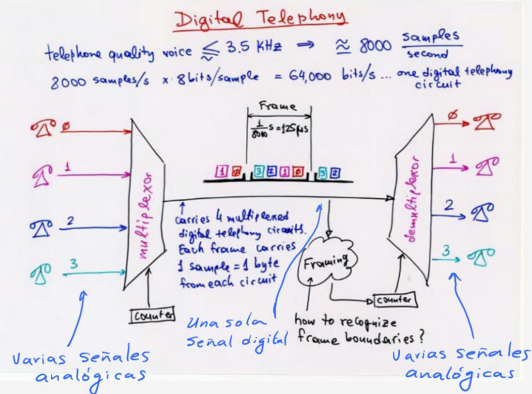
\includegraphics[scale=1]{Imagenes/Digital-telefono.png}
	\label{fig:Digital-telefono}
	%	\captionsetup{justification=raggedright,font={scriptsize,bf,it}}
	%	\caption*{fuente: \textcolor{
	%Orange}{Tomada de Wikipedia}}
\end{figure}

En telefonía al multiplexor a menudo se le llamó concentrador, ya que recibe muchas líneas y entrega pocas.
El multiplexor digital usado en la telefonía también incluía capacidades de conmutación. Era justamente la era de la conmutación de circuitos que consistía en cambiar la ventana de tiempo asignada a una llamada de modo que así cambiará el destinatario. \\

Una red más real requería usar centrales telefónicas para que una llamada pudiese llegar a cualquier destino. \\

\vspace{200px}
\begin{figure}[h!]
	\captionsetup{justification = raggedright, singlelinecheck = false}
	\caption{Modelo con las redes telefónicas} 
	\centering
	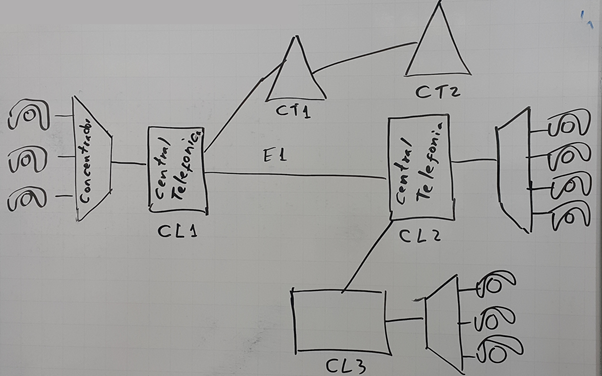
\includegraphics[scale=0.7]{Imagenes/Concentrador.png}
	\label{fig:Concentrador}
	%	\captionsetup{justification=raggedright,font={scriptsize,bf,it}}
	%	\caption*{fuente: \textcolor{
	%Orange}{Tomada de Wikipedia}}
\end{figure}

Al poco tiempo se complementó el modelo con las redes de transporte especializadas, inicialmente, en interconectar centrales telefónicas. La tecnología usada en esas redes se llama SDH (Synchronous Digital Hierarchy) y hoy sirven para interconectar todas las redes de voz y datos, mediante enlaces de fibra óptica, incluyendo cable submarino, enlaces de microondas y enlaces satelitales. \\

\begin{figure}[h!]
	\captionsetup{justification = raggedright, singlelinecheck = false}
	\caption{Red SDH} 
	\centering
	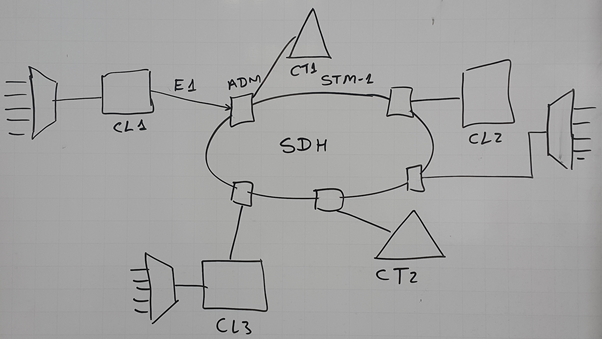
\includegraphics[scale=0.7]{Imagenes/SDH.png}
	\label{fig:SDH}
	%	\captionsetup{justification=raggedright,font={scriptsize,bf,it}}
	%	\caption*{fuente: \textcolor{
	%Orange}{Tomada de Wikipedia}}
\end{figure}

\section{MULTIACCESO POR DIVISIÓN DE FRECUENCIAS (FDMA)}
\subsection{Problema que justicia esta tecnología:}

Al comenzar la era de las comunicaciones móviles surgen diversos sistemas de primera generación 1G como: NMT (Nordic Mobile Telephone), AMPS (Advanced Mobile Phone System), TACS (Total Access Communication System), C-450, Radicom, RTMI, NTT. El reto principal consistía en lograr de muchos usuarios pudieran conectarse a una misma radiobase. La solución consistió simplemente en asignar una banda de frecuencias a cada llamada. \\

\begin{figure}[h!]
	\captionsetup{justification = raggedright, singlelinecheck = false}
	\caption{Ejemplo de multiacceso} 
	\centering
	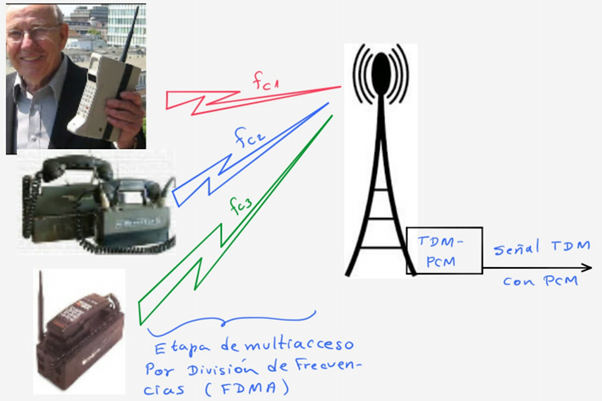
\includegraphics[scale=0.5]{Imagenes/Multiacceso.png}
	\label{fig:Multiacceso}
	%	\captionsetup{justification=raggedright,font={scriptsize,bf,it}}
	%	\caption*{fuente: \textcolor{
	%Orange}{Tomada de Wikipedia}}
\end{figure}

El multiacceso es la manera en que múltiples usuarios logran compartir un mismo recurso inalámbrico para resultar conectados a una misma radiobase. \\

\section{El Multiacceso por División de Tiempo (TDMA)}

Con FDMA solo las élites tenían acceso a las comunicaciones móviles, pues resultaban extremadamente costosas. Como ocurrió con la telefonía fija, la UIT ahora se propuso la meta de lograr que cada persona tuviese un  celular y eso requería una nueva revolución tecnológica para hacer más eficiente y flexible el uso del espectro. Surgieron entonces las comunicaciones móviles de Segunda Generación (2G). La novedad era esencialmente la implementación de TDMA. Como se deduce de la siguiente figura, el terminal de usuario debe preparar la señal digital para ir enviándola por una ventana de tiempo que se repite periódicamente.Surge así un nuevo tipo de canal para enviar información- \textbf{\textit{el canal de tiempo}}.\\

\vspace{400px}
\begin{figure}[h!]
	\captionsetup{justification = raggedright, singlelinecheck = false}
	\caption{Ejemplo de multiacceso} 
	\centering
	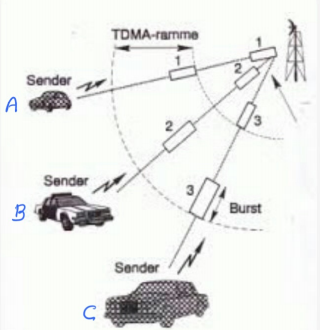
\includegraphics[scale=1]{Imagenes/Canal-tiempo.png}
	\label{fig:Canal-tiempo}
	%	\captionsetup{justification=raggedright,font={scriptsize,bf,it}}
	%	\caption*{fuente: \textcolor{
	%Orange}{Tomada de Wikipedia}}
\end{figure}

En la figura vemos que al usuario A ocupa el canal 1, el B el 2 y el C el 3. Con TDMA surgen los sistemas móviles de Segunda generación (2G) que se caracteriza por: ser digital, ser asequible, llevar voz y datos. Entre los sistemas 2G se tienen: GSM, D-AMPS (también conocido como sistema TDMA), cdma-one (también conocido como IS-95), PDC.\\


\section{Fundamentos de codificación del canal}

El capítulo 4 de este libro se dedica a un estudio más profundo de la codificación del canal. En el presente capítulo sólo se realiza un abrebocas, presentando el ejemplo más sencillo de codificación de canal con el fin de justificar la necesidad de usar técnicas de diversidad.

\subsection{Teorema de Shannon}

El Teorema de Shannon o Teorema de codificación del canal ruidoso (1948) establece las fronteras para la máxima información teórica que se puede transferir a un canal con un cierto nivel de ruido. Increíblemente, los últimos límites en la teoría de la información y codificación fueron determinados justo cuando esta ciencia nació, con los primeros artículos de Shannon. El resultado más conocido de Shannon es el teorema de la capacidad de un canal. El teorema establece que para muchas clases comunes de canal existe un parámetro que ha sido llamado Capacidad de Canal C, sobre el cual viajan códigos a una rata $R < C$ que pueden alcanzar transmisiones con cualquier grado de confiabilidad, pero estos códigos no existen para $R > C$.\\

El teorema también establece que para una canal de ancho de banda B (Hz) y afectado solo por ruido blanco aditivo gaussiano (AWGN del inglés Additive White Gaussian Noise), la capacidad C (en bps) solo depende de dos parámetros: el ancho de banda B y la relación señal a ruido SNR (del inglés Signal to Noise Relationship), así.\\

\begin{equation} \label{capseis_uno}
	C= Blog_2(1+SNR)
\end{equation}

Este teorema ha significado un reto para las siguientes generaciones de investigadores que se han enfrascado en lograr que sus algoritmos se acerquen al menos a ese límite establecido por Shannon. En los procesos de codificación y decodificación está en gran manera la clave para alcanzarlo. \\

\subsection{El proceso de codificación y decodificación digital del canal}

El problema de la codificación es planteado por el canal. Como ya  se ha dicho en otros capítulos los efectos del canal en el proceso de la comunicación es la razón por la cual aumenta constantemente el número de elementos o nuevos métodos de tratamiento de la información. Pareciera que con lo visto en capítulos anteriores, ya se ha visto todo sobre esos métodos, pero la realidad es que por más soluciones que se implementen siempre existirá la posibilidad de que la información llegue al destino con errores.\\

\begin{figure}[h!]
	\captionsetup{justification = raggedright, singlelinecheck = false}
	\caption{Relación entre transmisor, canal y receptor} 
	\centering
	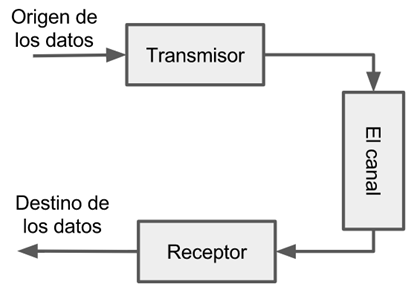
\includegraphics[scale=1]{Imagenes/Relacion-canal.png}
	\label{fig:Relacion-canal}
	%	\captionsetup{justification=raggedright,font={scriptsize,bf,it}}
	%	\caption*{fuente: \textcolor{
	%Orange}{Tomada de Wikipedia}}
\end{figure}

Entonces surgen varias preguntas:
\begin{itemize}
	\item [$\bullet$] ¿Es posible reconocer en qué momento se están presentando los errores?
	\item [$\bullet$] ¿Qué acciones es posible tomar cuando se han detectado errores?
\end{itemize}

La solución a estas preguntas está en lo que se conoce como Codificación del Canal. La idea es enviar junto con la información ciertos datos adicionales que permitan detectar la pérdida de bits, lo cual llamaremos codificación y se realiza en el transmisor. Finalmente, en el receptor se debe realizar el proceso de la detección de los errores, su corrección y la decodificación para recuperar los datos enviados, como se muestra en la siguiente figura.\\

\vspace{200px}
\begin{figure}[h!]
	\captionsetup{justification = raggedright, singlelinecheck = false}
	\caption{El proceso de codificación y decodificación } 
	\centering
	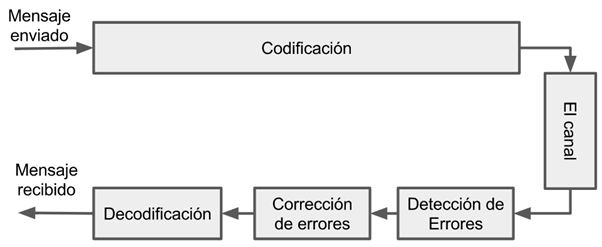
\includegraphics[scale=1]{Imagenes/Codificacion.png}
	\label{fig:Codificacion}
	%	\captionsetup{justification=raggedright,font={scriptsize,bf,it}}
	%	\caption*{fuente: \textcolor{
	%Orange}{Tomada de Wikipedia}}
\end{figure}

Los retos de la teoría de codificación del canal:
\begin{itemize}
	\item [$\bullet$] El primer reto consiste en poder corregir el máximo número de errores mientras se usa la mínima redundancia (rata) posible
	\item [$\bullet$] El segundo reto consiste en construir códigos que tengan procesos eficientes de codificación y decodificación
\end{itemize}

\section{El código de repetición }

Para presentarle rápidamente un ejemplo de codificación al lector, a continuación se analiza el ejemplo más sencillo de codificación. Consiste en transmitir 3 veces cada bit. Entonces se tiene una tabla de verdad, a la cual también se refieren como un diccionario

	\begin{table}[h!]
		\captionsetup{justification = raggedright,singlelinecheck = false}
		\caption{Alguna descripción.}
		\label{tabla:tabla10}
		\centering
		\scalebox{1}{
		\begin{tabular}{|c|c|}
			\hline
			\textbf{Bit de información} &\textbf{Palabra asignada} \\ \hline
			0 & 000  \rule[1mm]{0mm}{5mm}\\ \hline 
			1 & 111  \rule[1mm]{0mm}{5mm} \\ \hline
		\end{tabular}}
	\end{table}

En el receptor, para el ejemplo dado, se pueden recibir 8 posibles versiones de datos a interpretar. En el receptor podría usarse la siguiente tabla de verdad para interpretar la información útil:

\vspace{200px}
	\begin{table}[h!]
	\captionsetup{justification = raggedright,singlelinecheck = false}
	\caption{Alguna descripción.}
	\label{tabla:tabla11}
	\centering
	\scalebox{0.90}{
		\begin{tabular}{|c|c|c|}
			\hline
			\textbf{Tribits recibidos} & \textbf{Bit Interpretado} & \textbf{Número de Errores identificados} \\ \hline
			000 & 0 & 0  \rule[1mm]{0mm}{5mm}\\ \hline 
			001 & 0 & 1  \rule[1mm]{0mm}{5mm} \\ \hline
			010 & 0 & 1	 \rule[1mm]{0mm}{5mm} \\ \hline
			100 & 0 & 1	 \rule[1mm]{0mm}{5mm} \\ \hline
			111 & 1 & 0  \rule[1mm]{0mm}{5mm} \\ \hline
			110 & 1 & 1  \rule[1mm]{0mm}{5mm} \\ \hline
			101 & 1 & 1  \rule[1mm]{0mm}{5mm} \\ \hline
			011 & 1 & 1  \rule[1mm]{0mm}{5mm} \\ \hline
			
	\end{tabular}}
\end{table}

\textbf{Ventajas de esta codificación:} Es muy fácil codificar y decodificar.\\

\textbf{Desventaja:} Baja rata $ \frac{1}{3} $\\

Un ejemplo un poco mes avanzado se puede ver en el vídeo explicativo del siguiente enlace:\textcolor{blue}{\href{https://www.youtube.com/watch?v=0CLTy231Hsw}{Vídeo que explica un ejemplo de FEC}}

\section{Técnicas adicionales usadas en las comunicaciones móviles}

\subsection{Técnicas o esquemas de Diversidad}

El problema a resolver con estas técnicas puede ser planteado de la siguiente manera: \\

El Teorema de Shannon nos plantea un reto importante, que puede ser resuelto mediante técnicas de codificación del canal. Pero en un sistema de comunicaciones es muy común que los errores aparezcan concentrados de manera indeseada. Por ejemplo, cuando vimos el comportamiento de los niveles de potencia de la señal RF cuando se presenta el fenómeno de multitrayectoria, vimos que la señal puede presentar fuertes caídas, con respecto a la media. Supongamos que una caída de esas es debido al paso de carros entre el receptor y la radio base, el caso es que eso hace que se produzca una ràfaga de un volumen alto bits perdidos concentrados en un instante de tiempo. El volumen puede ser tan alto que los algoritmos de codificación del canal no tienen nada que hacer. Entonces diríamos que el Teorema de Shannon falla en estos casos?. La respuesta es que se requieren técnicas adicionales, como los esquemas de diversidad para lograr que los errores queden de alguna manera distribuidos uniformemente y la codificación del canal funcione mejor. \\

Los esquemas de diversidad se tratan de métodos para mejorar la recepción de una señal mensaje usando dos o más canales con diferentes características, pero usualmente sin agregar otra redundancia que la que pueden imprimir los mètodos de codificaciòn del canal. Desde este punto de vista, puede decirse que esta técnica es complementaria a los métodos de codificación del canal, para lograr que la codificación del canal sea más efectiva. Es una técnica común para combatir el desvanecimiento variable y las interferencias cocanal que experimentan las señales en su paso por un canal que producen ráfagas de errores. Se basan en que canales individuales experimentan diferentes niveles de desvanecimiento y de interferencia. La idea es transmitir y/o recibir múltiples versiones de la misma señal para hacerles un tratamiento en el receptor que permita obtener una mejor versión del mensaje que cuando se usa un solo canal. \\

\subsection{Diversidad de tiempo. Interleaving, FEC}

Se usa principalmente cuando el sistema de comunicación usa canales de tiempo, como ocurre al usar TDMA en un sistema de comunicaciones móviles, donde a la comunicación de un usuario le corresponde solo una ventana en el tiempo o Time-Slot dentro de un canal de frecuencia. Es el caso de las comunicaciones móviles digitales en general, pero el caso más claro son los sistemas de comunicaciones móviles de segunda generación (2G), los cuales usan, en la interfaz aire, PCM y  multiplexado por división de tiempo (TDM) como principal innovación con respecto al sistema de comunicaciones móviles de primera generación (1G) el cual usaba métodos analógicos en la interfaz aire.
Una señal TDM tiene muchos canales de tiempo, y resulta lógico pensar que cada uno de ellos pasa por diferentes condiciones de propagación. Por ejemplo, si la señal entre una radiobase y un usuario es interrumpida por el paso de algún obstáculo en medio de ellos, esto puede impactar a algunos canales de tiempo pero no a todos. En este caso toma sentido una técnica conocida como bit-interleaving que consiste en mezclar los bits de todos los canales de tiempo de manera que, si se pierde un canal de tiempo, no se pierdan todos los bits de unos ciertos time-slots sino que esa pérdida se reparta homogéneamente entre todos los usuarios, de modo que cada usuario pierda solo unos pocos bits. Ahora es cuando surge el reto de poder recuperar los pocos bits perdidos y cuando toma sentido otra técnica adicional conocida como Forward Error Correction (FEC). Esta consiste en agregar redundancia al mensaje, de manera previa o posterior al interleaving, para lograr reconocer en el receptor los bits perdidos y poder recuperarlos. El Interleaving evita entonces las ráfagas de errores, mejorando el desempeño de las técnicas FEC que son efectivas cuando hay pocos bits perdidos en cada canal de tiempo. Es importante notar que el Interleaving no significa enviar el mensaje de manera redundante, son las técnicas FEC las que introducen información que permita al receptor descubrir errores. Desde este punto de vista Interleaving y FEC son capas diferentes en un sistema de comunicaciones: la capa de interleaving se encarga de distribuir bits, la FEC de mantener un sistema capaz de corregir errores para lo cual en el transmisor se tiene una especie de codificador y en el receptor un decodificador. La cuestión es que la capa de FEC es más efectiva con el Interleaving y esta última tiene sentido sólo si se va a usar FEC, luego, van de la mano, pero queda claro que el interleaving no aplica redundancia, pero es el FEC quien lo hace. \\

\begin{figure}[h!]
	\captionsetup{justification = raggedright, singlelinecheck = false}
	\caption{Examples on the time diversity using the interleaving } 
	\centering
	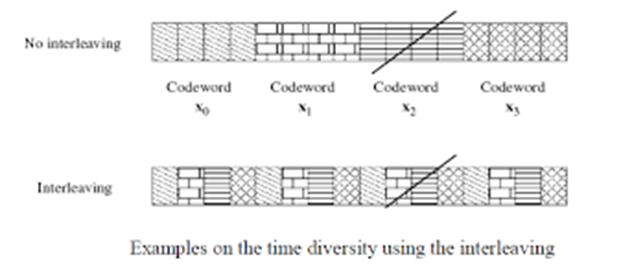
\includegraphics[scale=1]{Imagenes/Interrelacion.png}
	\label{fig:Interrelacion}
	%	\captionsetup{justification=raggedright,font={scriptsize,bf,it}}
	%	\caption*{fuente: \textcolor{
	%Orange}{Tomada de Wikipedia}}
\end{figure}

Pero el bit interleaving también tiene sentido incluso cuando la comunicación no se basa en TDMA. Supongamos que se tiene una comunicación digital inalámbrica solo entre dos puntos. Está claro que FEC va a funcionar mejor si los errores se concentran en ráfagas, va a ser más difícil corregir esos errores que cuando quedan repartidos de manera uniforme en el tiempo. \\

\section{Diversidad de espacio}

En los sistemas de comunicación cableada corresponde a la transmisión de una misma información por diferentes cables. En el caso de las comunicaciones inalámbricas es menos obvio pues no es la idea usar varios canales para la comunicación. Se trata más bien de una Diversidad de Antena, usando varias antenas para transmitir y/o recibir, lo cual debe ir seguido de técnicas de procesamiento digital para recuperar el mensaje a partir de esa diversidad que permite que cada antena aporte algo diferente que ayuda a la tarea de recuperación. Cuando el transmisor y el receptor usan varias antenas, se habla de técnicas MIMO (Multiple Input Multiple Output). Pero también se habla de macrodiversity o site diversity, cuando las antenas que participan en la comunicación están muy alejadas entre sí como es el caso de la existencia de varios puntos de acceso (access point) como se hace en las redes WLAN. Cuando esas distancias entre las antenas son menores a una longitud de onda se habla de microdiversidad y MIMO es un ejemplo de ella. Estas técnicas pueden combinarse adicionalmente con codificación para cada canal, con lo cual se habla de space-time coding (STC), así como con técnicas de beamforming para hacer que las antenas busquen a los usuarios, por ejemplo, cuando la concentración de usuarios cambia en el curso del día.   \\

\begin{figure}[h!]
	\captionsetup{justification = raggedright, singlelinecheck = false}
	\caption{Diversidad de espacio} 
	\centering
	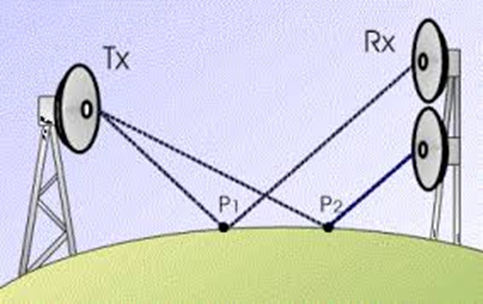
\includegraphics[scale=1]{Imagenes/Antenas-TX.png}
	\label{fig:Antenas-TX}
	%	\captionsetup{justification=raggedright,font={scriptsize,bf,it}}
	%	\caption*{fuente: \textcolor{
	%Orange}{Tomada de Wikipedia}}
\end{figure}
\vspace{200px}

\begin{figure}[h!]
	\captionsetup{justification = raggedright, singlelinecheck = false}
	\caption{Diversidad de espacio} 
	\centering
	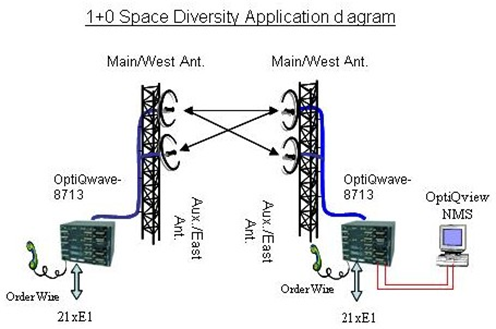
\includegraphics[scale=1]{Imagenes/Antenas-RX.png}
	\label{fig:Antenas-RX}
	%	\captionsetup{justification=raggedright,font={scriptsize,bf,it}}
	%	\caption*{fuente: \textcolor{
	%Orange}{Tomada de Wikipedia}}
\end{figure}

\subsection{Diversidad de polarización}

Consiste en enviar y/o recibir varias versiones de un mensaje usando diferentes \ 
polarizaciones de antena. Es en el fondo un caso especial de diversidad de espacio \ 
ya que usualmente se usan al menos dos antenas para darle a cada una polarización diferente. 

\begin{figure}[h!]
	\captionsetup{justification = raggedright, singlelinecheck = false}
	\caption{Ejemplo de diversidad de polarización} 
	\centering
	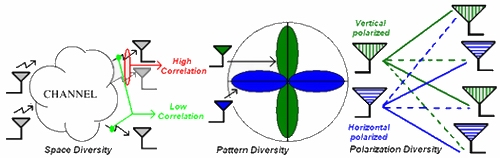
\includegraphics[scale=1]{Imagenes/Polarizacion.png}
	\label{fig:Polarizacion}
	%	\captionsetup{justification=raggedright,font={scriptsize,bf,it}}
	%	\caption*{fuente: \textcolor{
	%Orange}{Tomada de Wikipedia}}
\end{figure}

\subsection{Diversidad de frecuencias}	

El mensaje se transmite y/o recibe usando varios canales de frecuencia. Como en los casos anteriores, no necesariamente debe haber transmisión redundante, pues también es muy común la distribución premeditada de la información en varios canales. Supongamos un sistema de comunicaciones móviles donde el espectro disponible se ha dividido en sub-bandas A,B,C,D. Supongamos también que a un usuario se le asigna la subbanda A, pero en la práctica la información transmitida para todos los usuarios ha sido previamente mezclada, de modo que resulta repartida en todas las subbandas. Entonces, el usuario, en modo de recepción, deberá poder recibir todas las subbandas para poder pretender extraer lo que le corresponde. La técnica que más claramente se relaciona con este ejemplo es la que se conoce como OFDM usada en las comunicaciones móviles de Cuarta Generación (4G) y en la televisión digital. \\

\begin{figure}[h!]
	\captionsetup{justification = raggedright, singlelinecheck = false}
	\caption{Múltiples tuberías de capa física (PLP)} 
	\centering
	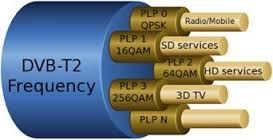
\includegraphics[scale=1]{Imagenes/DVB-T2.png}
	\label{fig:DVB-T2}
	%	\captionsetup{justification=raggedright,font={scriptsize,bf,it}}
	%	\caption*{fuente: \textcolor{
	%Orange}{Tomada de Wikipedia}}
\end{figure}

Otra posibilidad es el uso de la técnica de conocida como FHSS (Frequency Hopping Spread Spectrum), usada en las redes WIFI y Bluetooth.\\

\subsection{Diversidad de multi usuario}

Consiste en que el transmisor o radiobase agenda de manera oportunista al usuario, estudiando las condiciones del canal entre ella y todos los usuarios para seleccionar al usuario que tiene mejores cualidades para la comunicación. la idea es elegir el mejor instante para atender a cada usuario de la manera más óptima posible. 

\subsection{Diversidad cooperativa}

Se trata de una especie de diversidad de ganancia de antena que se alcanza usando antenas de otros usuarios o nodos.

\subsection{Diversidad de códigos}

Un ejemplo es lo que puede lograrse usando la técnica conocida como DS-SS (Direct Sequence Spread Spectrum) que predomina en las comunicaciones móviles de tercera generación (3G) que facilita el uso redundante del ancho de banda.

\section{La Duplexación}

Es la solución que permite a los usuarios conectados a una radiobase mantener una comunicación bidireccional. \\

Duplexación por División de Frecuencias (FDD) se usa una banda de frecuencias para la información que va desde el usuario a la radiobase, es decir para el \textbf{ Enlace de subida o up-link} y otra banda para la información que va desde la radiobase al usuario. es decir \textbf{el Enlace de bajada o Dowlink}. \\

FDD es el método de Duplexación más usado desde el comienzo de las comunicaciones móviles hasta el día de hoy. A manera de ejemplo, la figura \ref{fig:Bandas} muestra la \
distribución de la banda conocida como 1900MHz, entre los operadores móviles establecidas en Colombia. Allí vemos por ejemplo que a la banda A destinada para up-link le corresponde la banda A’ destinada para Downlink. \
Obsérvese también que en medio de esas grandes bandas existe una central que sirve de guarda, pero que hoy día busca ser aprovechada mediante otro tipo de Duplexación, \textbf{La Duplexación por División de Tiempo (TDD).} \\

\vspace{50px}

\begin{figure}[h!]
	\captionsetup{justification = raggedright, singlelinecheck = false}
	\caption{Banda 1900 como posibilidad de ser aprovechada por duplexación por division de tiempo TDD.} 
	\centering
	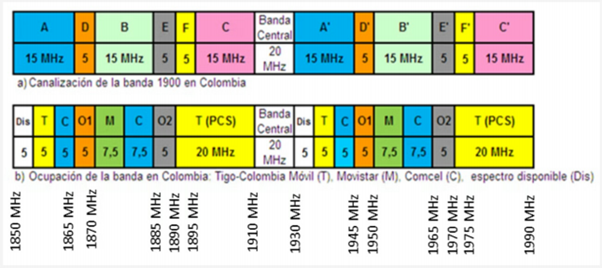
\includegraphics[scale=1]{Imagenes/Bandas.png}
	\label{fig:Bandas}
	%	\captionsetup{justification=raggedright,font={scriptsize,bf,it}}
	%	\caption*{fuente: \textcolor{
	%Orange}{Tomada de Wikipedia}}
\end{figure}


La figura \ref{fig:FDMA} resume la distribución de bandas de frecuencia de los términos estudiados.

%\vspace{200px}
\begin{figure}[h!]
	\captionsetup{justification = raggedright, singlelinecheck = false}
	\caption{Resumen de FDMA-FD, TDMA-FDD, FDMA-TDD. } 
	\centering
	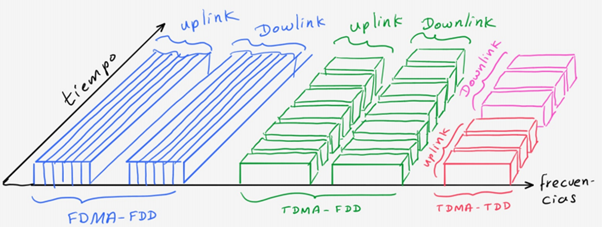
\includegraphics[scale=1]{Imagenes/FDMA.png}
	\label{fig:FDMA}
	%	\captionsetup{justification=raggedright,font={scriptsize,bf,it}}
	%	\caption*{fuente: \textcolor{
	%Orange}{Tomada de Wikipedia}}
\end{figure}

\vspace{200px}
\subsection{La celda y la radiobase}


\begin{figure}[h!]
	\captionsetup{justification = raggedright, singlelinecheck = false}
	\caption{La celda y la radiobase} 
	\centering
	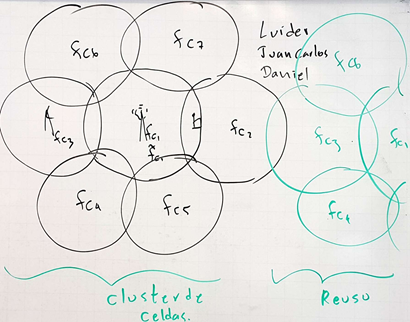
\includegraphics[scale=1]{Imagenes/Cluster.png}
	\label{fig:Cluster}
	%	\captionsetup{justification=raggedright,font={scriptsize,bf,it}}
	%	\caption*{fuente: \textcolor{
	%Orange}{Tomada de Wikipedia}}
\end{figure}

\subsection{El reuso}

\subsection{El handoff}

\section{Spread Spectrum (SS) y el Multiacceso por División de Códigos (CDMA)}

Es la tecnología que hace posible el multiplexado por división de códigos (CDM) y consecuentemente el multiacceso por división de códigos (CDMA), que dio origen a un sistema 2G conocido como CDMA-ONE, que inicialmente competía con los sistemas GSM y D-AMPS. La batalla en 2G por el mercado mundial la ganó GSM debido a la gran expansión que logró al provenir de la unión de todos los países europeos. Pero CDMA-ONE logró demostrar que era la tecnología que permitía el uso más flexible del espectro. \\

\textit{Problema que impulsa la tecnología Spread Spectrum:} La necesidad no está originalmente en las comunicaciones móviles, sino simplemente en la comunicación entre dos puntos. Por ejemplo, entre el piloto de un avión militar y el comando en tierra. Durante la segunda guerra mundial era ideal poder emitir señales que el enemigo no pudiese detectar. La idea consiste en lograr distribuir la energía de la señal útil en una banda muy ancha, para que su PSD se parezca a la del ruido blanco. Así el enemigo solo detectará en sus equipos de medición la presencia de ruido blanco. Hoy esta tecnología es ampliamente usada para la implementación de \textit{enlaces de microondas en bandas de frecuencia de uso libre}, las cuales son muy congestionadas. En este sentido, SS permite establecer enlaces incluso en bandas que ya están ocupadas sin interferirlas. \\ 

\vspace{200px}
\begin{figure}[h!]
	\captionsetup{justification = raggedright, singlelinecheck = false}
	\caption{SIN NOMBRE} 
	\centering
	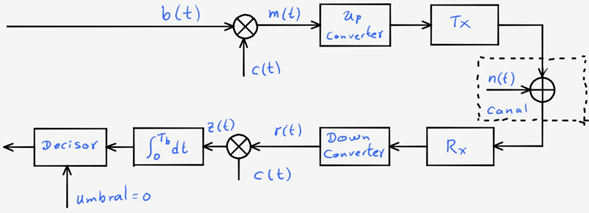
\includegraphics[scale=1]{Imagenes/Diagrama-TX.png}
	\label{fig:Diagrama-TX}
	%	\captionsetup{justification=raggedright,font={scriptsize,bf,it}}
	%	\caption*{fuente: \textcolor{
	%Orange}{Tomada de Wikipedia}}
\end{figure}

Para su análisis resulta útil usar un sistema equivalente en banda base, como el siguiente:\\


\begin{figure}[h!]
	\captionsetup{justification = raggedright, singlelinecheck = false}
	\caption{SIN NOMBRE} 
	\centering
	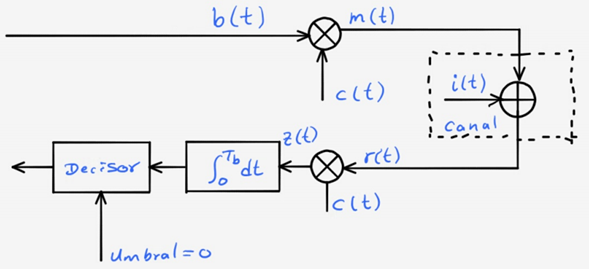
\includegraphics[scale=1]{Imagenes/Diagrama-RX.png}
	\label{fig:Diagrama-RX}
	%	\captionsetup{justification=raggedright,font={scriptsize,bf,it}}
	%	\caption*{fuente: \textcolor{
	%Orange}{Tomada de Wikipedia}}
\end{figure}

$b_t$ es usualmente una señal binaria con $R_b= \dfrac{1}{T_b}$, pero puede ser cualquier señal digital banda base, por ejemplo la envolvente compleja 8-PSK, con $R_{sym}= 1/ T_{sym}$.\\

$c(t)$ es una señal de ruido que se caracteriza por tomar valores en 1 y -1 cada $T_c$, donde  $T_{c}<<T_{b}$ o $T_{c}<<T_{sym}$.

\vspace{200px}

\begin{figure}[h!]
	\captionsetup{justification = raggedright, singlelinecheck = false}
	\caption{Señales de ejemplo.} 
	\centering
	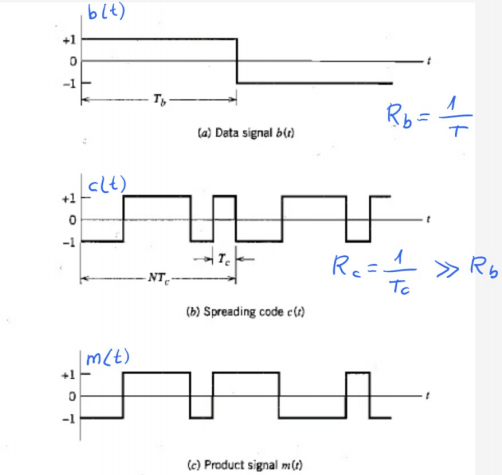
\includegraphics[scale=1]{Imagenes/Data.png}
	\label{fig:Data}
	%	\captionsetup{justification=raggedright,font={scriptsize,bf,it}}
	%	\caption*{fuente: \textcolor{
	%Orange}{Tomada de Wikipedia}}
\end{figure}

Veamos la PSD de estas señales:

\begin{figure}[h!]
	\captionsetup{justification = raggedright, singlelinecheck = false}
	\caption{PSD de las señales.} 
	\centering
	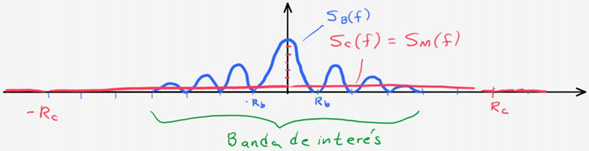
\includegraphics[scale=1]{Imagenes/Banda-interes.png}
	\label{fig:Banda-interes}
	%	\captionsetup{justification=raggedright,font={scriptsize,bf,it}}
	%	\caption*{fuente: \textcolor{
	%Orange}{Tomada de Wikipedia}}
\end{figure}

Podemos observar que:

\begin{itemize}
	\item [$\bullet$] La PSD de la señal $c(t) y m(t)=b(t)*c(t)$ se expande hasta una frecuencia        $N=\frac{R_c}{R_b}$ veces mayor, a la vez que cae en altura, hasta el punto que, dentro de una banda de interés para la transmisión/recepción $S_c(f)$ y $S_m(f)$ resultan siendo similares a la del ruido blanco. Por lo anterior, c(t) aunque es binaria bipolar es considerada una señal de ruido.
	\item [$\bullet$] Es ideal que $c(t)$ sea totalmente aleatoria para que tenga la PSD mostrada, pero esto es difícil de lograr ya que $c(t)$ debe ser conocida tanto en el transmisor como en le receptor.
	\item [$\bullet$] En la práctica, $c(t)$ es generada por un dispositivo conocido como GENERADOR DE SECUENCIAS DE PSEUDORUIDO. La idea es lograr que exista un generador idéntico en la parte transmisora y en la receptora. Esta limitación hace que $c(t)$ no tenga características completamente aleatorias, al punto que incluso $c(t)$ resulta siendo una señal periódica, aunque el periodo puede ser tan grande que esta periodicidad puede ser ignorada en el análisis. Por esta razón, $c(t)$ es en la práctica una señal o secuencia de pseudoruido.
	\item [$\bullet$] Entre más grande será el factor de dispersión (SF- del inglés “Spreading Factor”)       $N=\frac{R_c}{R_b}$ o $N=\frac{R_c}{R_sym}$, menos se notará la señal emitida m(t) en receptores diferentes al nuestro, los cuales la verán más bien como ruido blanco.
\end{itemize}

\textit{Análisis de la parte receptora:}\\

Es importante resaltar que la señal $i(t)$ que en el canal se suma de manera indeseada a nuestra señal útil $m(t)$ puede ser, más que ruido blanco, potentes señales de otras emisiones indeseadas, es decir, interferencias que producen otros sistemas de comunicación de la banda de frecuencia de nuestro sistema. Por eso, revisaremos el peor caso de la PSD de una señal $i(t)$ como se muestra en la figura \ref{fig:Banda-triangulo} \\

\begin{figure}[h!]
	\captionsetup{justification = raggedright, singlelinecheck = false}
	\caption{Peor de los casos de la señal i(t).} 	\centering
	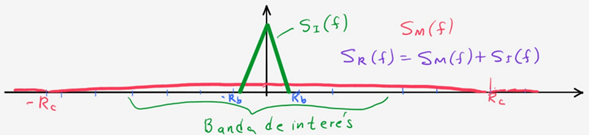
\includegraphics[scale=1]{Imagenes/Banda-triangulo.png}
	\label{fig:Banda-triangulo}
	%	\captionsetup{justification=raggedright,font={scriptsize,bf,it}}
	%	\caption*{fuente: \textcolor{
	%Orange}{Tomada de Wikipedia}}
\end{figure}

\begin{equation} \label{capseis_dos}
r(t)= m(t)+ i(t);    z(t)= r(t)*c(t) 
\end{equation}

\begin{equation} \label{capseis_tres}
z(t)=[m(t)+ i(t)]*c(t)=  [b(t)*c(t)+i(t)]*c(t) 
\end{equation}

\begin{equation} \label{capseis-cuatro}
z(t)=b(t)*c^{2}(t)+i(t)*c(t)
\end{equation}

Si $c(t)$ es binaria bipolar de amplitud 1, entonces $c^{2}(t)=1$.

\begin{equation} \label{capseis-cinco}
z(t)=\underbrace{b(t)+i(t)}_{Nuestro \ mensaje \ se \ recupera   } * \underbrace{c(t)}_{ La \ senal\ de \ interferencia \ se \ dispersa \ en \ las \ frecuencias}
%%\overbrace{x+\underbrace{y+z}_{2} +w}^{4}
\end{equation}

\vspace{200px}
\begin{figure}[h!]
	\captionsetup{justification = raggedright, singlelinecheck = false}
	\caption{Señal b(t).} 
	\centering
	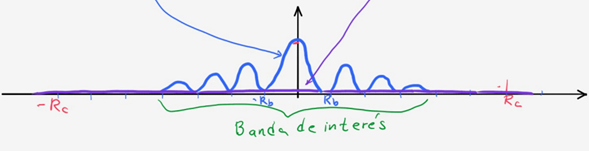
\includegraphics[scale=1]{Imagenes/Banda-seno.png}
	\label{fig:Banda-sena}
	%	\captionsetup{justification=raggedright,font={scriptsize,bf,it}}
	%	\caption*{fuente: \textcolor{
	%Orange}{Tomada de Wikipedia}}
\end{figure}

Finalmente, un filtro de acoplamiento y un decisor de umbral permiten recuperar la señal $b(t)$.

\subsection{Tipos de Spread Spectrum}

Hoy se habla de dos grandes tipos de espectro disperso:

\begin{itemize}
	\item [$\bullet$] El que hace uso de las secuencias de pseudoruido, que es justo el tema explicado anteriormente y se conoce mejor como DS - SS (Direct Sequence Spread Spectrum).
	\item [$\bullet$] El que hace uso de saltos de frecuencias y que se conoce mejor como FH – SS (Frequency Hopping Spread Spectrum).
\end{itemize}

\textbf{El Multiacceso por División de códigos (CDMA)}

DS-CDMA (Direct Sequence Code Division Multiaccess).\\

Este tipo de multiacceso fue usado por la empresa estadounidense Qualcomm en el sistema móvil 2G conocido como CDMA - ONE. Este sistema pronto perdió la batalla en los mercados, pero demostró que esta forma de multiacceso era más flexible y más eficiente que TDMA en comunicaciones que combinan voz y datos.\\

CDMA usa tecnología DS-SS y a menudo se conoce también como DS – CDMA. La figura  \ref{fig:Cuadrado-link} muestra cómo se usa el espectro cuando se usa CDMA.

\begin{figure}[h!]
	\captionsetup{justification = raggedright, singlelinecheck = false}
	\caption{Distribucion del espectro con CDMA.} 
	\centering
	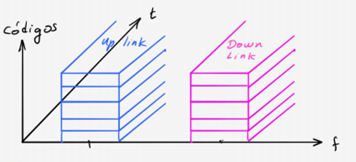
\includegraphics[scale=1]{Imagenes/Cuadrado-link.png}
	\label{fig:Cuadrado-link}
	%	\captionsetup{justification=raggedright,font={scriptsize,bf,it}}
	%	\caption*{fuente: \textcolor{
	%Orange}{Tomada de Wikipedia}}
\end{figure}

\section{Multiacceso por División de Códigos de banda ancha (WCDMA)}

Finalizado el siglo XX la UIT se propuso comenzar el año 2000 con una nueva revolución en las comunicaciones: lograr que cada persona, independientemente de su condición económica, tuviese la posibilidad de estar siempre conectado, desde cualquier lugar, en cualquier momento, mediante cualquier terminal y en cualquier situación.

\subsection{Convergencia de las comunicaciones}

Hasta ese momento, las redes de telecomunicaciones se desarrollaban para prestar servicios independientes. Por ejemplo, la telefonía fija, permitía: hacer llamadas, usar buzones de llamadas, llamadas bipartidas, etc. Pero solo entre usuarios de telefonía fija. Por supuesto se podía llamar desde un teléfono fijo a un móvil, pero los costos eran exorbitantemente mayores. Lo mismo ocurría con las redes de datos, tenían servicios propios, que si bien era posible acceder por medio de la telefonía fija o la móvil, se hacía con una muy baja calidad y unos costos absurdos. \\

Retos tecnológicos: \\

\begin{itemize}
	\item [$\bullet$] Organizar el núcleo de todas las redes, ahora ese núcleo se llamaría  \textit{REDES DE NUEVA GENERACIÓN (NGN)}.
\end{itemize}

\begin{figure}[h!]
	\captionsetup{justification = raggedright, singlelinecheck = false}
	\caption{Redes clásicas y redes de nueva generación.} 
	\centering
	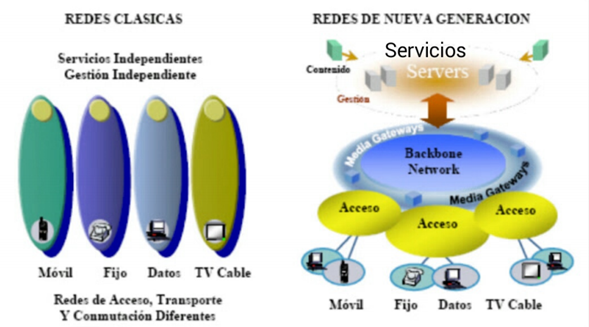
\includegraphics[scale=1]{Imagenes/Redes-retos.png}
	\label{fig:Redes-retos}
	%	\captionsetup{justification=raggedright,font={scriptsize,bf,it}}
	%	\caption*{fuente: \textcolor{
	%Orange}{Tomada de Wikipedia}}
\end{figure}

El impacto principal de las NGN consistía en posibilitar el desarrollo de servicios comunes a todas las posibilidades de los usuarios.


\begin{itemize}
	\item [$\bullet$] Retos políticos: En Colombia, la política nacional se consolida en la \textit{ley 1341 de 2009} ley 1341 de 2009 y en el \textit{ Plan de Gobierno Vive Digital}.
	\item [$\bullet$] Acuerdo internacional para producir un sistema único para las comunicaciones móviles, las cuales eran la clave para lograr la revolución trazada.
\end{itemize}

\subsection{El UMTS}

Hoy ese sistema \textit{UMTS (Universal Mobile Telecommunication System)}, que corresponde a \textit{la tercera generación de comunicaciones móviles (3G)}. Algunos también le llaman WCDMA ya que implementa la tecnología de multiacceso conocida como  \textit{Multiacceso por División de Códigos de banda ancha}, para lograr que los usuarios puedan establecer comunicaciones con requerimientos flexibles de uso de las bandas de frecuencia disponibles.\\

\subsection{IMT-2000}

Es la recomendación que emitió la UIT para impulsar las comunicaciones móviles 3G. Fue escrito con apoyo del 3GPP (Third Generation Partnership Project) – un conjunto de entidades interesadas en estos avances que incluyen: proveedores de tecnología, operadores, etc. El número 2000 hace referencia al esperanzador año 2000 y también a la necesidad de sumar bandas de frecuencias para el nuevo sistema, cercanas a los 2000 MHz. 2000 kbps también era la meta establecida para la velocidad de datos que podrían tener los usuarios desde sus terminales móviles usando la nueva Interfaz aire. IMT (International Mobile Telecommunications) significa la necesidad de un sistema único mundial.\\

\subsection{WCDMA:}

El sistema de tercera generación UMTS usa CDMA de banda ancha (WCDMA) que se diferencia de CDMA en los siguientes aspectos:\\

Se usan bandas de frecuencia de ancho 5MHz, que es notablemente mayor al usado en CDMA-ONE.\\

Se usan códigos de Walsh para distinguir los usuarios. Se trata de una familia de señales que tienen una forma similar a las secuencias de pseudoruido, pero son todas ortogonales entre sí. La siguiente figura muestra un ejemplo de ocho Funciones de Walsh.\\

\begin{figure}[h!]
	\captionsetup{justification = raggedright, singlelinecheck = false}
	\caption{Funciones de Walsh.} 
	\centering
	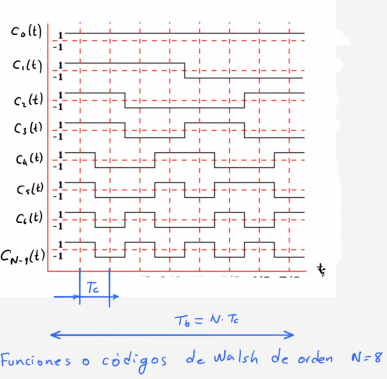
\includegraphics[scale=1]{Imagenes/Funciones-codigo.png}
	\label{fig:Funciones-codigo}
	%	\captionsetup{justification=raggedright,font={scriptsize,bf,it}}
	%	\caption*{fuente: \textcolor{
	%Orange}{Tomada de Wikipedia}}
\end{figure}

$N$ es el número de diferentes códigos de Walsh. Coincide con el número máximo de usuarios simples. También coincide con el número de chips en l duración de un bit. Por tanto           $SF=N x N= 2^{n}$, donde n es un entero.\\

El término “usuario simple” se ha usado porque en principio un usuario podría llegar a usar varios códigos en la práctica. \\

Debido a su ortogonalidad se cumple que: \\

\begin{equation} \label{capseis_seis}
\int_{T_{b}}^0 C_{n}(t)*C_{k}(t)dt={0, n diferente de k 1, n=k}
\end{equation}

Gracias a esto los usuarios no se interfieren entre sí. \\

Ejercicio: Comprobar si el código $C_{2}(t)$ y el $C_{5}(t)$ son ortogonales en el periodo $T_{b}$.

\begin{figure}[h!]
	\captionsetup{justification = raggedright, singlelinecheck = false}
	\caption{ Ejercicios funciones de Walsh.} 
	\centering
	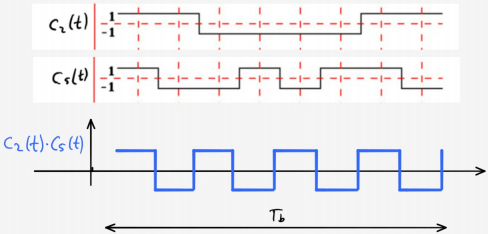
\includegraphics[scale=1]{Imagenes/Funcion-dos.png}
	\label{fig:Funciones-dos}
	%	\captionsetup{justification=raggedright,font={scriptsize,bf,it}}
	%	\caption*{fuente: \textcolor{
	%Orange}{Tomada de Wikipedia}}
\end{figure}

\begin{equation} \label{capseis_siete}
\int_{T_{b}}^0 C_{2}(t)*C_{5}(t)dt=0
\end{equation}

Así que $C_{2}(t)$ y $C_{5}(t)$ son ortogonales en ese periodo. \\

Ejercicio: Tenemos el siguiente sistema de comunicación. 4 usuarios envían un mensaje cada uno a una radio base, donde esos 4 mensajes deben ser extraídos a partir de la señal $s(t)$.\\

\vspace{200px}
\begin{figure}[h!]
	\captionsetup{justification = raggedright, singlelinecheck = false}
	\caption{Sistemas de comunicaciones.} 
	\centering
	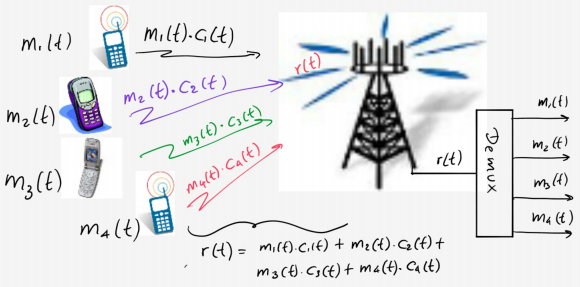
\includegraphics[scale=1]{Imagenes/Demux.png}
	\label{fig:Demux}
	%	\captionsetup{justification=raggedright,font={scriptsize,bf,it}}
	%	\caption*{fuente: \textcolor{
	%Orange}{Tomada de Wikipedia}}
\end{figure}

Para obtener cada señal $m_{k}(t)$ en el demux se usa el esquema de la página 3 para cada una de esas señales. Veamos el caso del usuario k=2. Dentro del demux se halla $r(t)*c_{2}(t)$ \\

\begin{equation} \label{capseis_ocho}
z_{2}(t)=[m_{1}(t)*c_{1}(t)*c_{2}(t)]+ [m_{2}(t)*c_{2}(t)*c_{2}(t)]+ [m_{3}(t)*c_{3}(t)*c_{2}(t)]+ [m_{4}(t)*c_{4}(t)*c_{2}(t)]
\end{equation}

Es importante aclarar que durante el tiempo, cada una de las señales $m_{k}(t)$ tiene un valor constante $A_{k}$. Veamos un ejemplo para $m_{2}(t)$. Si $m_{2}(t)$ es la siguiente 

\begin{figure}[h!]
	\captionsetup{justification = raggedright, singlelinecheck = false}
	\caption{Ejemplo $m_{2}(t)$.} 
	\centering
	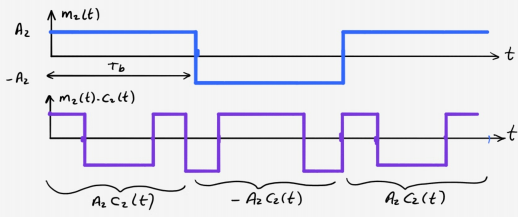
\includegraphics[scale=1]{Imagenes/Linea-cuadro.png}
	\label{fig:Linea-cuadro}
	%	\captionsetup{justification=raggedright,font={scriptsize,bf,it}}
	%	\caption*{fuente: \textcolor{
	%Orange}{Tomada de Wikipedia}}
\end{figure}

\begin{equation} \label{capseis_nueve}
\int_{T_{b}}^0 z(t)dt= \int_{T_{b}}^0 m_{1}(t)*c_{1}(t)*c_{2}(t)dt+ \int_{T_{b}}^0 m_{2}(t)*c_{2}^{2}(t)dt + \int_{T_{b}}^0 m_{1}(t)*c_{3}(t)*c_{2}(t)dt + \int_{T_{b}}^0 m_{4}(t)*c_{4}(t)*c_{2}(t)dt
\end{equation}

\begin{equation} \label{capseis_diez}
\int_{T_{b}}^0 z(t)dt= A1 \int_{T_{b}}^0 *c_{1}(t)*c_{2}(t)dt+ A2 \int_{T_{b}}^0 + A3 \int_{T_{b}}^0 c_{3}(t)*c_{2}(t)dt + A4 \int_{T_{b}}^0 c_{4}(t)*c_{2}(t)dt
\end{equation}

Debido a la ortogonalidad entre los códigos en el intervalo Tb tenemos que:

\begin{equation} \label{capseis_once}
\int_{T_{b}}^0 z(t)dt = A2* T_{b} => \dfrac{1}{T_{b}} \int_{T_{b}}^0 z(t)dt = A2
\end{equation}

\textit{En conclusión:} Vemos que para cada ventana de tiempo de duración $T_{b}$ es posible encontrar el valor de cada mensaje sin ningún tipo de afectación de parte de los mensajes de los otros usuarios. \\

Por el hecho de usar códigos ortogonales este tipo de técnica de espectro ensanchado se conoce como Orthogonal Variable Spreading Factor (OVSF) y es considerado como una forma de CDMA. Esto es debido a que cada código de Walsh tiene un ancho de espectro diferente y por lo tanto se produce un Sf diferente a mensaje, pero nunca superior a SF=N. \\

Se combina TDMA con CDMA. 

\begin{figure}[h!]
	\captionsetup{justification = raggedright, singlelinecheck = false}
	\caption{Distribución del espectro combinando TDMA con CDMA.} 
	\centering
	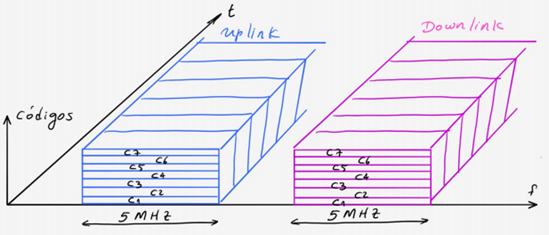
\includegraphics[scale=1]{Imagenes/TDMA.png}
	\label{fig:TDMA}
	%	\captionsetup{justification=raggedright,font={scriptsize,bf,it}}
	%	\caption*{fuente: \textcolor{
	%Orange}{Tomada de Wikipedia}}
\end{figure}

La figura \ref{fig:TDMA} muestra cómo se aprovecha la banda de frecuencias destinada a una radio base. En UMTS, esa banda es de 5MHz. Surge la pregunta lógica ¿Cómo se podría representar en esa gráfica el uso que las diferentes radio bases hacen del espectro? Recordemos que en los sistemas basados en TDMA (como GSM y D-AMPS) la banda de frecuencias asignada a un operador es dividida en N subbandas centradas en las frecuencias de las portadoras fc1, fc2, fc3…, fn que se asignan a N celdas aledañas de modo que no se presenten interferencias perceptibles por los usuarios de cualquier celda. Se conforma entonces, un clúster de N celdas, como se muestra en la figura \ref{fig:Cluster-movil}: 

\vspace{200px}
\begin{figure}[h!]
	\captionsetup{justification = raggedright, singlelinecheck = false}
	\caption{Cluster de N celdas.} 
	\centering
	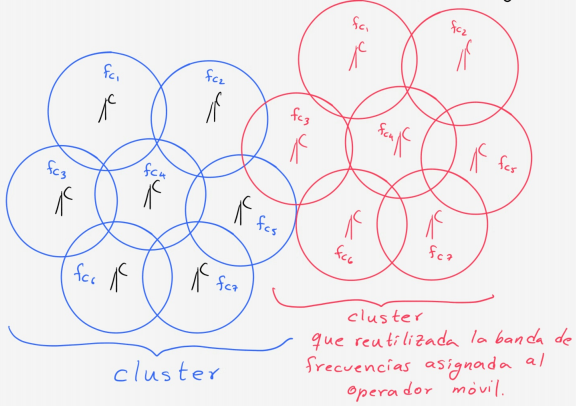
\includegraphics[scale=1]{Imagenes/Cluster-movil.png}
	\label{fig:Cluster-movil}
	%	\captionsetup{justification=raggedright,font={scriptsize,bf,it}}
	%	\caption*{fuente: \textcolor{
	%Orange}{Tomada de Wikipedia}}
\end{figure}

\subsection{El reúso en UMTS}

Se usan secuencias de pseudoruido (PN – del inglés Pseudo - noise) para distinguir las celdas. 

%\vspace{200px}
\begin{figure}[h!]
	\captionsetup{justification = raggedright, singlelinecheck = false}
	\caption{El reúso en UMTS} 
	\centering
	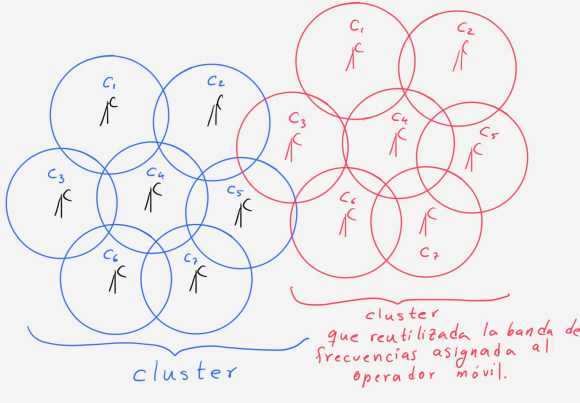
\includegraphics[scale=0.7]{Imagenes/FDD.png}
	\label{fig:FDD}
	%	\captionsetup{justification=raggedright,font={scriptsize,bf,it}}
	%	\caption*{fuente: \textcolor{
	%Orange}{Tomada de Wikipedia}}
\end{figure}

De modo que, admirablemente, con UMTS un operador móvil podría contar mínimamente con 10MHz (5MHz para el Uplink y 5 para el Downlink, si usa duplexación FDD (la mayoría lo hace)). No necesita subbandas de frecuencias para conformar clusters de celdas, pues \textit{UMTS reutiliza una banda de 5MHz mediante códigos de Pseudoruido}. \\

Cabe aclarar que una banda tiene en todo caso una capacidad limitada de trafico dada por la limitación de potencia de los transmisores usados principalmente en las radio bases. Cada usuario conectado demanda parte de esa energía que emite la radio base de manera proporcional a la velocidad de datos del servicio que el usuario utiliza. Por ello, no es raro que los operadores tengan en la práctica varias bandas UMTS, Cuando esto ocurre, pudiera decirse que el multiacceso en UMTS combina CDMA con TDMA y con FDMA, aunque a la combinación de todo eso, en la práctica, se conoce simplemente como WCDMA. \\

\subsection{Respiración de las celdas en UMTS}

Este tema se ha dejado se ha dejado para que el estudiante lo investigue y ponga a prueba los conocimientos adquiridos para comprender fácilmente otros. Durante esta investigación no olvide que: una radio base y también un terminal tienen potencia limitada; a diferencia de otros sistemas. UMTS busca atender con calidad similar a un usuario que está cerca de la radio base y a otro que está lejos de ella.\\

\section{OFDM – OFDMA}

OFDM es un multiplexado por División de Frecuencias (FDM), que usa portadoras que son ortogonales entre sí. La figura \ref{fig:OFDM} muestra 4 portadoras ortogonales.\\

\begin{figure}[h!]
	\captionsetup{justification = raggedright, singlelinecheck = false}
	\caption{OFDM} 
	\centering
	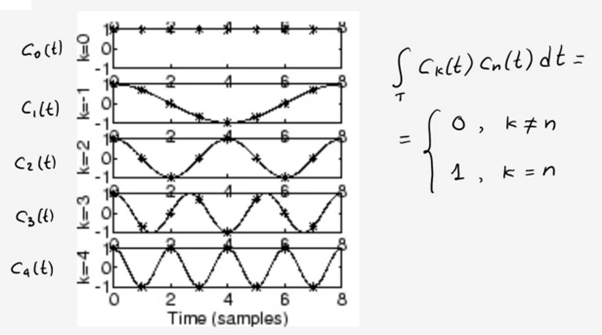
\includegraphics[scale=0.9]{Imagenes/OFDM.png}
	\label{fig:OFDM}
	%	\captionsetup{justification=raggedright,font={scriptsize,bf,it}}
	%	\caption*{fuente: \textcolor{
	%Orange}{Tomada de Wikipedia}}
\end{figure}

Todas las señales senoidales cuyas frecuencias sean múltiplo entero de una cierta frecuencia $f_{0}$, son ortogonales entre sí.

\subsection{Realización práctica de OFDM}

Haber descubierto que una señal OFDM se puede producir usando el algoritmo FFT (Fast Fourier Transform) es una de las causas del amplio uso que ha tenido en las comunicaciones de Cuarta Generación (4G), que se han materializado en el sistema LTE (Long Term Evolution).

\begin{figure}[h!]
	\captionsetup{justification = raggedright, singlelinecheck = false}
	\caption{sistema LTE (Long Term Evolution)} 
	\centering
	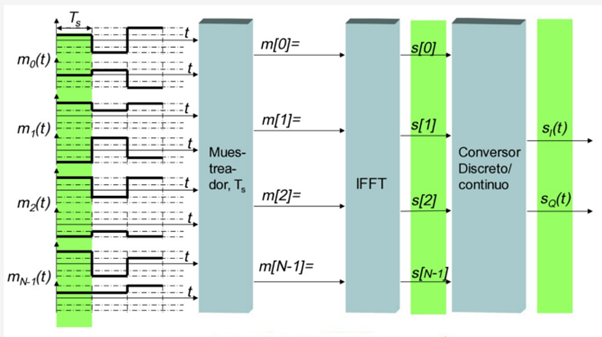
\includegraphics[scale=0.9]{Imagenes/Multiplexar.png}
	\label{fig:Multiplexar}
	%	\captionsetup{justification=raggedright,font={scriptsize,bf,it}}
	%	\caption*{fuente: \textcolor{
	%Orange}{Tomada de Wikipedia}}
\end{figure}

$m_{0}(t)$, $m_{1}(t)$, … , $m_{N-1}(t)$  \ 
son las señales a multiplexar, ellas pueden ser señales reales binarias, pero también pueden ser señales digitales moduladas en su versión de envolvente compleja, como se muestra en la figura, donde cada señal tiene una componente I y una Q y por lo tanto trae símbolos de duración Ts. \\

El muestreador hace que solo una muestra por cada símbolo pase al siguiente bloque llamado IFFT (Inverse Fast Fourier Transform). Este bloque ejecuta la operación inversa de Representación en Series de Fourier Discreta:

\begin{equation} \label{capseis_doce}
\sum_{k=0}^{N-1}m[k]e^{j \frac{2 \pi kn}{N}} ,n=[0, N-1]
\end{equation}

La figura \ref{fig:Conversor-discreto} muestra el paso del primer símbolo de cada mensaje por los bloques del multiplexor. La IFFT recibe ese paquete y entrega N muestras de la señal multiplexada.

\vspace{200px}
\begin{figure}[h!]
	\captionsetup{justification = raggedright, singlelinecheck = false}
	\caption{Paso del primer símbolo por los bloques del multiplexor.} 
	\centering
	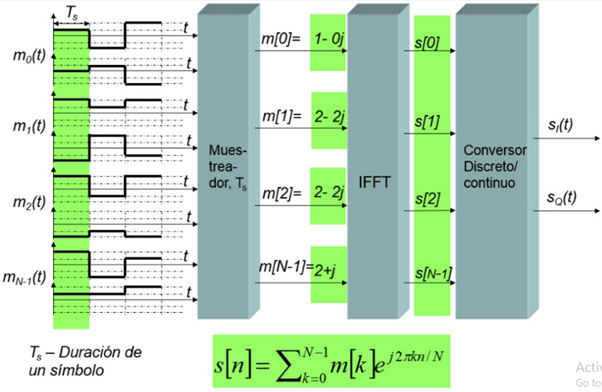
\includegraphics[scale=0.9]{Imagenes/Conversor-discreto.png}
	\label{fig:Conversor-discreto}
	%	\captionsetup{justification=raggedright,font={scriptsize,bf,it}}
	%	\caption*{fuente: \textcolor{
	%Orange}{Tomada de Wikipedia}}
\end{figure}

Lo mismo se repite para el segundo símbolo como lo muestra la figura \ref{fig:Conversor-continuo}.

\begin{figure}[h!]
	\captionsetup{justification = raggedright, singlelinecheck = false}
	\caption{Paso del segundo símbolo por los bloques del multiplexor.} 
	\centering
	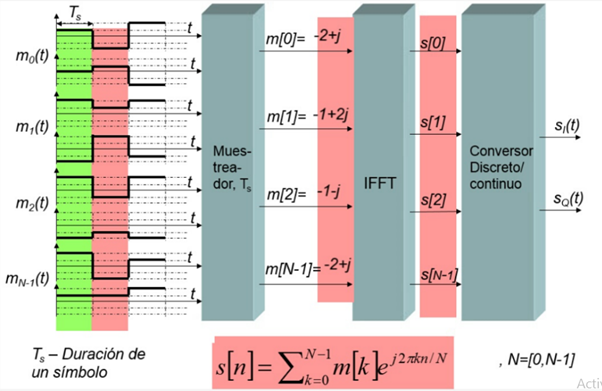
\includegraphics[scale=0.9]{Imagenes/Conversor-continuo.png}
	\label{fig:Conversor-continuo}
	%	\captionsetup{justification=raggedright,font={scriptsize,bf,it}}
	%	\caption*{fuente: \textcolor{
	%Orange}{Tomada de Wikipedia}}
\end{figure}

Se produjo otro paquete de N muestras de la señal s[n]. Esas muestras van siendo organizadas en serie y convertidas en una señal continua por el bloque “Conversor Discreto/Continuo”.

\vspace{200px}
\begin{figure}[h!]
	\captionsetup{justification = raggedright, singlelinecheck = false}
	\caption{Paso del N símbolo hasta llegar al bloque “Conversor Discreto/Continuo”. } 
	\centering
	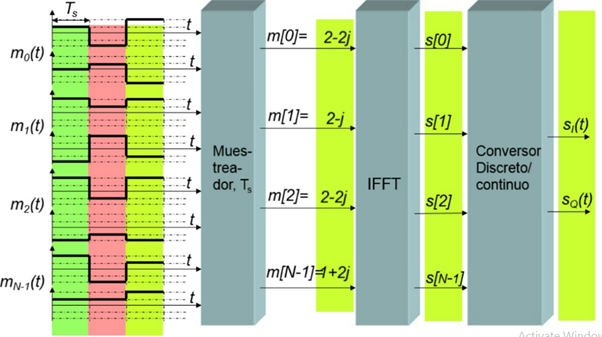
\includegraphics[scale=0.9]{Imagenes/Muestreador.png}
	\label{fig:Muestreador}
	%	\captionsetup{justification=raggedright,font={scriptsize,bf,it}}
	%	\caption*{fuente: \textcolor{
	%Orange}{Tomada de Wikipedia}}
\end{figure}

Como la señal discreta es:

\begin{equation} \label{capseis_trece}
s[n]= \sum_{k=0}^{N-1}m[k]e^{j \frac{2 \pi kn}{N}} ,n=[0, N-1]
\end{equation}

Es importante notar que con un sola muestra $m[k]$ de todos los usuarios se obtienen N muestras de la señal $s[n]$. Eso significa que durante un periodo N, la muestra $m[k]$ se mantiene constante. Luego, $s[n]$ varía N veces más rápido que $m[k]$. Sea $m[k]$,n una versión de $m[k]$ sobre muestreada N veces, osea que por cada valor $m[k]$ se produce $m[k,0]=m[k]$, , $m[k,1]=m[k]$,  ... , $m[k,N-1]=m[k]$, entonces se justifica la siguiente expresión.

\begin{equation} \label{capseis_catorce}
s[n]= \sum_{k=0}^{N-1}m[k,n]e^{j \frac{2 \pi kn}{N}} ,n=[0, N-1]
\end{equation}

Entonces puede deducirse que si esa señal se hace pasar por un conversor discreto a continua, se obtiene:

\begin{equation} \label{capseis_quince}
s[n]= \sum_{k=0}^{N-1}m_{k}(t)e^{j2\pi kf_{0}t} , f_{0}= \frac{1}{T_{s}}, t= [0, \infty]
\end{equation}

Esta fórmula nos revela que esta interconexión es equivalente a la figura \ref{fig:Aliasing}.

\vspace{200px}
\begin{figure}[h!]
	\captionsetup{justification = raggedright, singlelinecheck = false}
	\caption{Efecto de Aliasing.} 
	\centering
	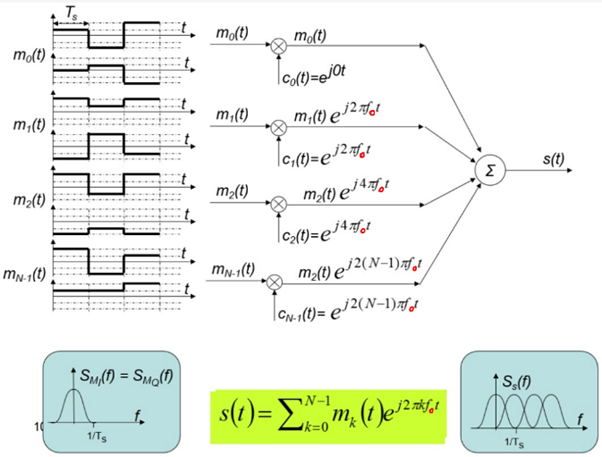
\includegraphics[scale=0.9]{Imagenes/Aliasing.png}
	\label{fig:Aliasing}
	%	\captionsetup{justification=raggedright,font={scriptsize,bf,it}}
	%	\caption*{fuente: \textcolor{
	%Orange}{Tomada de Wikipedia}}
\end{figure}

Efecto del aliasing. \\

Es importante tener en cuenta los efectos del aliasing que se presenta con las señales senoidales discretas, como se muestra en la siguiente figura, en la cual puede deducirse que $c_{7}[n]=c_{1}[n]$, donde * se usa para señalar que es el conjugado. Si estas dos señales se miran en un plano complejo, veremos que son vectores rotantes que giran a una misma velocidad, pero en direcciones contrarias. Por lo tanto también puede decirse que:

\begin{equation} \label{capseis_diesiseis}
c_{7}[n]=e^{j2 \pi 7n/N}=C_{-1}[n]=e^{j2 \pi n/N}
\end{equation}

Lo mismo ocurre entre $c_{6}[n]$ y $c_{2}[n]$, así como entre $c_{5}[n]$ y $c_{3}[n]$.

\vspace{200px}
\begin{figure}[h!]
	\captionsetup{justification = raggedright, singlelinecheck = false}
	\caption{Efecto aliasing.} 
	\centering
	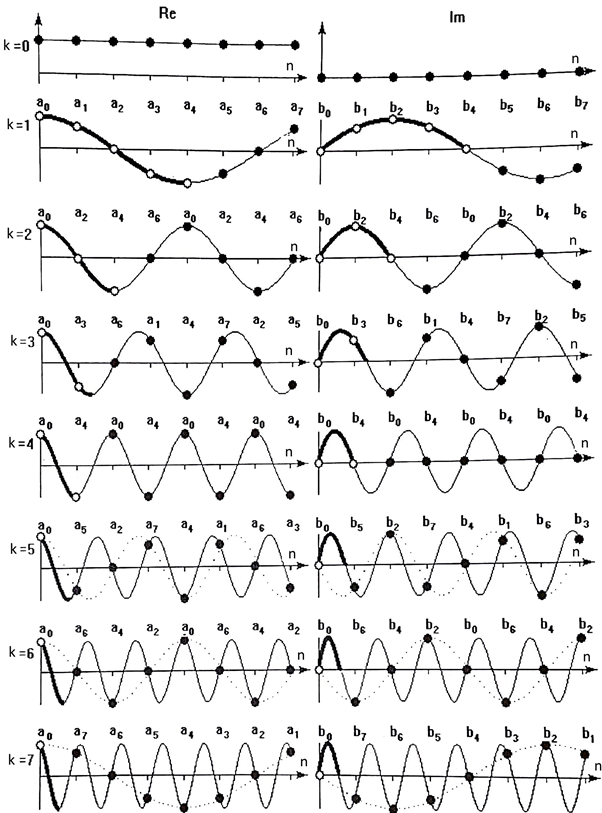
\includegraphics[scale=0.6]{Imagenes/Efecto-aliasing.png}
	\label{fig:Efecto-aliasing}
	%	\captionsetup{justification=raggedright,font={scriptsize,bf,it}}
	%	\caption*{fuente: \textcolor{
	%Orange}{Tomada de Wikipedia}}
\end{figure}

Como el USRP no mira las frecuencias que están entre 0 Hz y la frecuencia de muestreo $F_{s}$Hz, sino entre $-F_{s}/2$ y $+F_{s}/2$, equivale a decir que solo reconoce la existencia de las portadoras $c_{-N/2}[n]$, … $c_{-1}[n]$, $c_{0}[n]$, $c_{1}[n]$, … , $c_{N/2}[n]$. Por esta razón, el espectro OFDM se obtiene centrado en la frecuencia cero como se muestra en la siguiente figura tomada de GNU Radio. 